\documentclass[11pt,a4paper]{article}
\usepackage[spanish,es-nodecimaldot]{babel}	% Utilizar español
\usepackage[utf8]{inputenc}					% Caracteres UTF-8
\usepackage{graphicx}						% Imagenes
\usepackage[hidelinks]{hyperref}			% Poner enlaces sin marcarlos en rojo
\usepackage{fancyhdr}						% Modificar encabezados y pies de pagina
\usepackage{float}							% Insertar figuras
\usepackage[textwidth=390pt]{geometry}		% Anchura de la pagina
\usepackage[nottoc]{tocbibind}				% Referencias (no incluir num pagina indice en Indice)
\usepackage{enumitem}
\usepackage[T1]{fontenc}
\usepackage{amsmath}

% Configuracion de encabezados y pies de pagina
\pagestyle{fancy}
\lhead{Vladislav Nikolov Vasilev}
\rhead{Aprendizaje Automático}
\lfoot{Grado en Ingeniería Informática}
\cfoot{}
\rfoot{\thepage}
\renewcommand{\headrulewidth}{0.4pt}		% Linea cabeza de pagina
\renewcommand{\footrulewidth}{0.4pt}		% Linea pie de pagina

\newcommand{\eout}{$E_{\text{out}}$}
\newcommand{\ein}{$E_{\text{in}}$}

\begin{document}
\pagenumbering{gobble}

% Pagina de titulo
\begin{titlepage}

\begin{minipage}{\textwidth}

\centering


\includegraphics[scale=0.5]{img/ugr.png}\\

\textsc{\Large Aprendizaje Automático\\[0.2cm]}
\textsc{GRADO EN INGENIERÍA INFORMÁTICA}\\[1cm]

\noindent\rule[-1ex]{\textwidth}{1pt}\\[1.5ex]
\textsc{{\Huge PRÁCTICA 2\\[0.5ex]}}
\textsc{{\Large Programación\\}}
\noindent\rule[-1ex]{\textwidth}{2pt}\\[3.5ex]

\end{minipage}

\vspace{0.5cm}

\begin{minipage}{\textwidth}

\centering

\textbf{Autor}\\ {Vladislav Nikolov Vasilev}\\[2.5ex]
\textbf{Rama}\\ {Computación y Sistemas Inteligentes}\\[2.5ex]
\vspace{0.3cm}


\includegraphics[scale=0.3]{img/etsiit.jpeg}

\vspace{0.7cm}
\textsc{Escuela Técnica Superior de Ingenierías Informática y de Telecomunicación}\\
\vspace{1cm}
\textsc{Curso 2018-2019}
\end{minipage}
\end{titlepage}

\pagenumbering{arabic}
\tableofcontents
\thispagestyle{empty}				% No usar estilo en la pagina de indice

\newpage

\setlength{\parskip}{1em}

\section{\textsc{Ejercicio sobre la complejidad de H y el ruido}}
\noindent En este ejercicio debemos aprender la dificultad que introduce la aparición de ruido en las
etiquetas a la hora de elegir la clase de funciones más adecuada. Haremos uso de tres funciones
ya programadas:

\begin{itemize}
	\item $simula\_unif(N, dim, rango)$, que calcula una lista de N vectores de dimensión $dim$.
	Cada vector contiene $dim$ números aleatorios uniformes en el intervalo $rango$.
	\item $simula\_gaus(N, dim, sigma)$, que calcula una lista de longitud N de vectores de
	dimensión $dim$, donde cada posición del vector contiene un número aleatorio extraido de una
	distribucción Gaussiana de media 0 y varianza dada, para cada dimension, por la posición
	del vector $sigma$.
	\item $simula\_recta(intervalo)$, que simula de forma aleatoria los parámetros, $v = (a, b)$
	de una recta, $y = ax + b$, que corta al cuadrado $[-50, 50] \times [-50, 50]$.
\end{itemize}

\subsection*{Apartado 1}
\addcontentsline{toc}{subsection}{Apartado 1}

\noindent Dibujar una gráfica con la nube de puntos de salida correspondiente.

\begin{enumerate}[label=\textit{\alph*})]
	\item Considere $N = 50$, $dim = 2$, $rango = [-50, +50]$ con $simula\_unif(N, dim, rango)$.
\end{enumerate}

Como el código de la función $simula\_unif$ se ha proporcionado, no se va a mostrar su funcionamiento
porque se supone que ya es conocido. Habiendo dicho esto, se procede a mostrar los datos generados:

\begin{figure}[H]
\centering
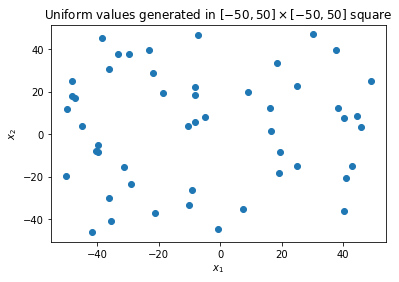
\includegraphics[scale=0.53]{img/simula_unif.png}
\caption{Datos generados por la función $simula\_unif(N, dim, rango)$ con $N = 50$, $dim = 2$,
$rango = [-50, +50]$}
\end{figure}

\begin{enumerate}[resume,label=\textit{\alph*})]
	\item Considere $N = 50$, $dim = 2$ y $sigma = [5, 7]$ con $simula\_gaus(N, dim, sigma)$.
\end{enumerate}

De nuevo, como en el caso anterior, como ya se ha proporcionado la función $simula\_gaus$, no se va
a mostrar su funcionamiento porque se supone que ya es conocido. Así que, con esto en mente, podemos
mostrar los siguientes puntos generados:

\begin{figure}[H]
\centering
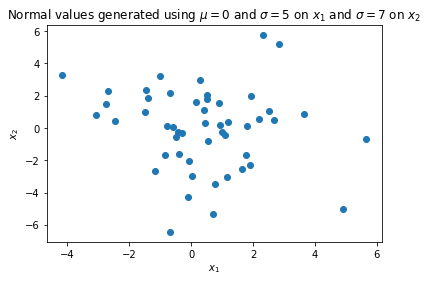
\includegraphics[scale=0.6]{img/simula_gaus.png}
\caption{Datos generados por la función $simula\_gaus(N, dim, sigma)$ con $N = 50$, $dim = 2$ y
$sigma = [5, 7]$}
\end{figure}

\subsection*{Apartado 2}
\addcontentsline{toc}{subsection}{Apartado 2}

\noindent Con ayuda de la función $simula\_unif()$ generar una muestra de puntos 2D a los
que vamos añadir una etiqueta usando el signo de la función $f(x, y) = y - ax - b$, es decir
el signo de la distancia de cada punto a la recta simulada con $simula\_recta()$.

\begin{enumerate}[label=\textit{\alph*})]
	\item Dibujar una gráfica donde los puntos muestren el resultado de su etiqueta, junto
	con la recta usada para ello. (Observe que todos los puntos están bien clasificados
	respecto de la recta).
\end{enumerate}

Para realizar esto, se nos ha proporcionado la función $simula\_recta()$ desde el principio, con lo
cuál no la vamos a comentar, ya que se supone conocida. Para clasificar los puntos, vamos a utilizar
una función llamada $f(x, y, a, b)$, donde $x$ es la coordenada $X$ del punto, $y$ la coordenada $Y$,
$a$ la pendiente de la recta simulada anteriormente y $b$ el termino independiente. Esta función
también se ha proporcionado, con lo cuál no se mostrará su implementación porque, de nuevo, se supone
conocida.

Los puntos generados, junto con la recta, son los siguientes:

\begin{figure}[H]
\centering
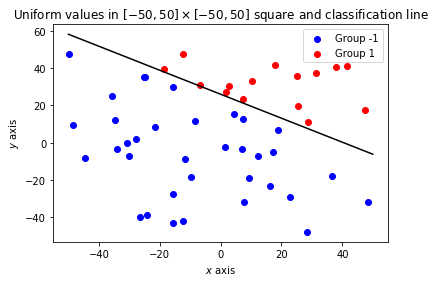
\includegraphics[scale=0.6]{img/data_line_no_noise.png}
\caption{Gráfica de puntos generados uniformemente con la recta que separa las dos clases.}
\end{figure}

Adicionalmente, para ver que la clasificación es la correcta, se ha calculado el ratio de puntos
clasificados correcta e incorrectamente mediante una función, la cuál se puede ver a continuación:

\begin{figure}[H]
\centering
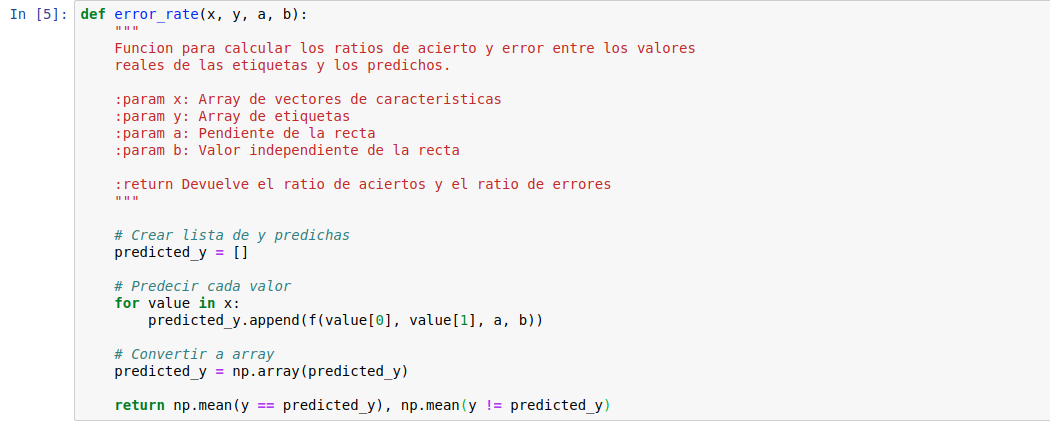
\includegraphics[scale=0.4]{img/error_rate.png}
\caption{Función para el cálculo del ratio de aciertos y errores.}
\end{figure}

Los resultados obtenidos, como se espera en este caso ya que no hay ruido en la muestra, son los
siguientes:

\begin{figure}[H]
\centering
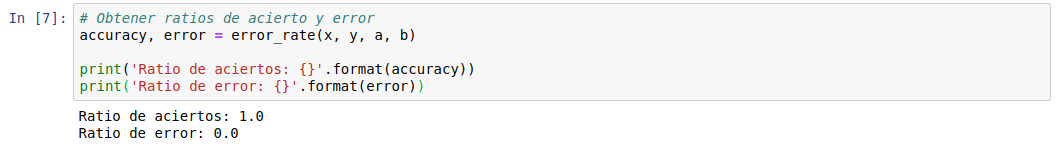
\includegraphics[scale=0.4]{img/error_no_noise.png}
\caption{Ratios de acierto y error obtenidos de la muestra sin ruido.}
\end{figure}

\begin{enumerate}[resume,label=\textit{\alph*})]
	\item Modifique de forma aleatoria un 10\% etiquetas positivas y otro 10\% de negativas
	y guarde los puntos con sus nuevas etiquetas. Dibuje de nuevo la gráfica anterior.
	(Ahora hay puntos mal clasificados respecto de la recta)
\end{enumerate}

Para insertar ruido en la muestra, de forma proporcional a la cantidad de etiquetas de las distintas
clases que tenemos, nos hemos ayudado de la siguiente función:

\begin{figure}[H]
\centering
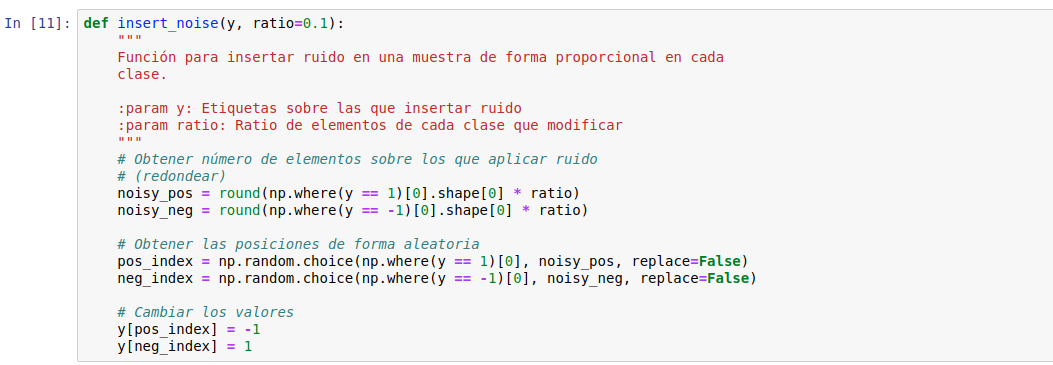
\includegraphics[scale=0.4]{img/insert_noise.png}
\caption{Función para insertar ruido en una muestra de datos.}
\end{figure}

Al aplicar esta función sobre nuestras etiquetas, obtenemos los siguientes datos:

\begin{figure}[H]
\centering
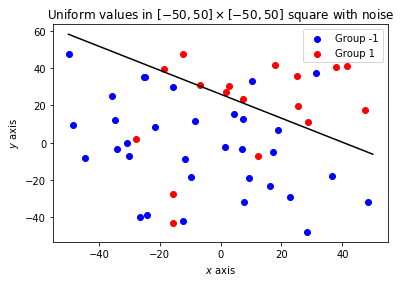
\includegraphics[scale=0.6]{img/data_line_noise.png}
\caption{Gráfica de puntos generados uniformemente con ruido junto con la recta que los separa.}
\end{figure}

Como se puede ver, como había un mayor número de datos con etiqueta $-1$, se han modificado más
elementos de esta clase, siendo este número de elementos modificados proporcional respecto al número
de elementos totales de la clase.

Como era de esperarse, al haber modificado las etiquetas, los ratios de aciertos y error se han
visto modificados, dejándolos de la siguiente forma:

\begin{figure}[H]
\centering
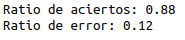
\includegraphics[scale=0.7]{img/rates_noise.png}
\caption{Ratios de acierto y error obtenidos de la muestra con ruido.}
\end{figure}

\subsection*{Apartado 3}
\addcontentsline{toc}{subsection}{Apartado 3}
\noindent Supongamos ahora que las siguientes funciones definen la frontera de clasificación
de los puntos de la muestra en lugar de una recta:

\begin{enumerate}
	\item \label{itm:f1} $f(x, y) = (x - 10)^2 + (y - 20)^2 - 400$
	\item \label{itm:f2} $f(x, y) = 0.5(x + 10)^2 + (y - 20)^2 - 400$
	\item \label{itm:f3} $f(x, y) = 0.5(x - 10)^2 + (y + 20)^2 - 400$
	\item \label{itm:f4} $y - 20x^2 - 5x + 3$
\end{enumerate}

\noindent Visualizar el etiquetado generado en 2\textit{b} junto con cada una de las gráficas de cada
una de las funciones. Comparar las formas de las regiones positivas y negativas de estas nuevas
funciones con las obtenidas en el caso de la recta ¿Son estas funciones más complejas
mejores clasificadores que la función lineal? ¿En qué ganan a la función lineal? Explicar el
razonamiento.

Para ayudarnos con la visualización de los datos, hemos utilizado una función ya proporcionada,
con lo cuál no vamos a discutir como funciona. En vez de eso, veamos cómo son las funciones 
anteriores una vez que se han implementado:

\begin{figure}[H]
\centering
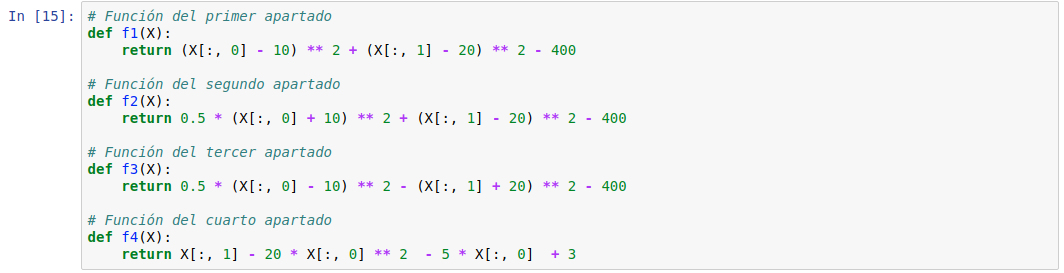
\includegraphics[scale=0.4]{img/functions.png}
\caption{Funciones implementadas en Python.}
\end{figure}

Estas funciones están pensadas para que se modifiquen todos los datos a la vez y se devuelva la
función aplicada a éstos.

Para calcular estos ratios, nos hemos ayudado de la siguiente función, la cuál ha sido parametrizada
para que pueda recibir cualquiera de las funciones anteriores, predecir las etiquetas y devolver
los correspondientes ratios:

\begin{figure}[H]
\centering
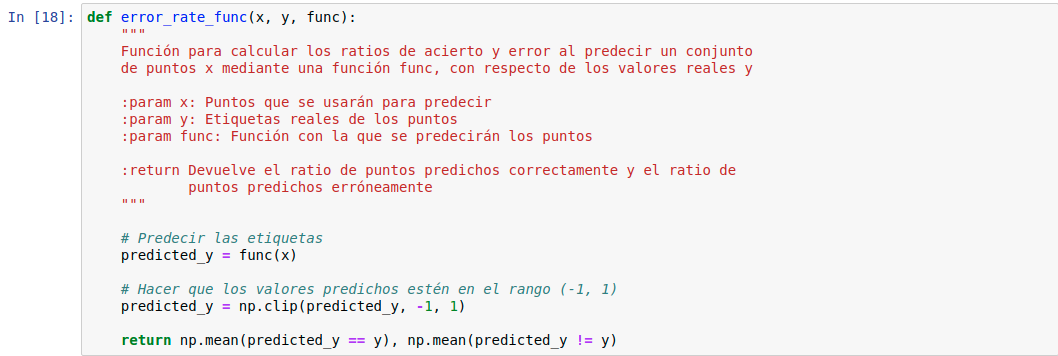
\includegraphics[scale=0.4]{img/error_rate_func.png}
\caption{Función para calcular las tasas de aciertos y error para las nuevas funciones.}
\end{figure}

A continuación, se presentan las gráficas de las funciones junto con los valors de los ratios
de aciertos y error:

\begin{figure}[H]
\centering
\begin{minipage}{.5\textwidth}
	\centering
	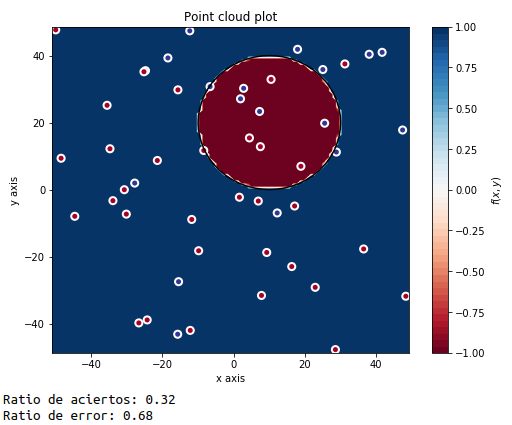
\includegraphics[scale=0.35]{img/f1.png}
	\caption{Gráfica y ratios de \ref{itm:f1}.}
\end{minipage}%
\begin{minipage}{.5\textwidth}
	\centering
	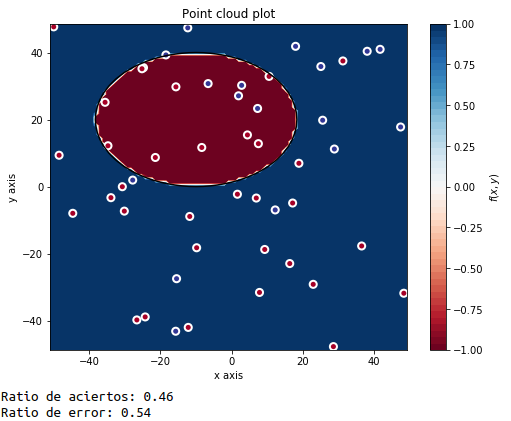
\includegraphics[scale=0.35]{img/f2.png}
	\caption{Gráfica y ratios de \ref{itm:f2}.}
\end{minipage}
\end{figure}

\begin{figure}[H]
\centering
\begin{minipage}{.5\textwidth}
	\centering
	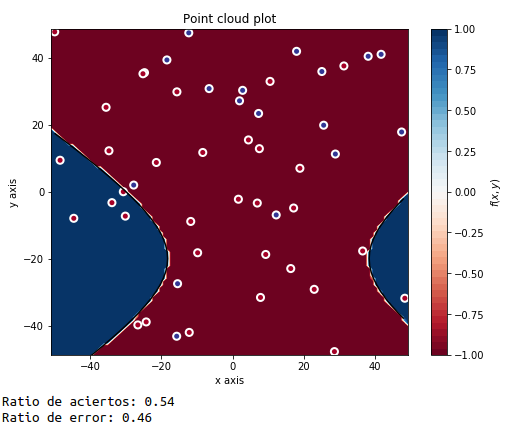
\includegraphics[scale=0.35]{img/f3.png}
	\caption{Gráfica y ratios de \ref{itm:f3}.}
\end{minipage}%
\begin{minipage}{.5\textwidth}
	\centering
	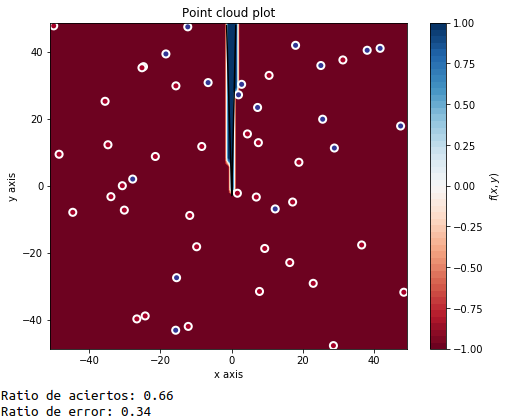
\includegraphics[scale=0.35]{img/f4.png}
	\caption{Gráfica y ratios de \ref{itm:f4}.}
\end{minipage}
\end{figure}

Como se puede ver, son funciones más complejas que las lineales. Algunas de ellas son figuras
geométricas, como circunferencias o elipses (correspondientes a las funciones \ref{itm:f1} y
\ref{itm:f2}). Estas funciones serían capaces de explicar datos muy complejos, datos con los que
las funciones lineales tendrían problemas, debido a que no son linealmente separables mediante
una recta. Por ejemplo, si una clase estuviese dentro de otra, se podría usar perfectamente una
función como \ref{itm:f1} o \ref{itm:f2}.

Comparándolas con la recta, las regiones positivas y negativas cambian. En el caso de la recta, todo
lo que había debajo de ella se supone que es negativo (aunque luego no sea así debido a la presencia
de ruido). En estos nuevos casos, encontramos por ejemplo que las regiones negativas están dentro
de las positivas (funciones \ref{itm:f1} y  \ref{itm:f2}), las regiones positivas están en los
extremos laterales (función \ref{itm:f3}) o son tan pequeñas que casi no existen o parecen una
parabola (caso de la función \ref{itm:f4}).

A pesar de esto, las funciones no parecen ser demasiado buenas, ya que en todos los casos los ratios
de aciertos son menores que los de la función lineal (recordemos que su ratio de aciertos era
$0.88$). Esto se debe a que, aunque los datos presenten un cierto ruido, se pueden llegar a separar
mejor utilizando una recta en vez de algo mucho más complejo como una elipse o dividiendo el espacio
en regiones como en el caso de \ref{itm:f3}.

También hay que considerar que en este caso estamos cogiendo directamente funciones, sin entrenar
ningún tipo de modelo para intentar ajustarlas a los datos. A lo mejor haciendo esto se podrían
obtener algunos resultados un poco mejores en algunas de las funciones, pero como existe ruido en la
muestra, es muy difícil dar con la función adecuada y que tenga el mínimo error. Además, en caso de
encontrarla, por haber recurrido a una clase de funciones muy compleja por ejemplo, nos podríamos
encontrar con el caso de \textit{overfitting}, lo cuál es un problema gravísimo y nada deseable.

En resumen, las funciones no lineales tienen sus puntos fuertes debido a que pueden explicar ciertos
tipos de muestras mejor de lo que lo haría una función lineal, pero no siempre son la solución a
nuestros problemas. Pueden darse casos, como por ejemplo este, que la función lineal le gane a todas
las no lineales, debido a que sea más fácil dividir los datos mediante una recta. Hay que ser muy
consciente de qué tipo de función elegir en cada momento. Por ejemplo, un comportamiento no lineal en
algunas carcterísticas nos podría indicar que sería mejor intentar recurrir a alguna función no lineal
que a una lineal para resolver el problema. Sin embargo, antes de recurrir a los modelos no lineales,
podemos asegurarnos comprobando alguna información como por ejemplo el sesgo y la varianza que nuestro
modelo lineal se queda corto para explicar los datos, teniendo en cuenta siempre que no se debe hacer
\textit{overfitting} con los datos disponibles.

\section{\textsc{Modelos Lineales}}

\subsection*{Apartado 1}
\addcontentsline{toc}{subsection}{Apartado 1}

\noindent \textbf{Algoritmo Perceptrón}: Implementar la función
$ajusta\_PLA(datos, label, max\_iter, vini)$ que calcula el hiperplano solución a un problema de
clasificación binaria usando el algoritmo PLA. La entrada $datos$ es una matriz donde cada item con
su etiqueta está representado por una fila de la matriz, $label$ el vector de etiquetas (cada etiqueta
es un valor $+1$ o $-1$), $max\_iter$ es el número máximo de iteraciones permitidas y $vini$ el valor
inicial del vector. La función devuelve los coeficientes del hiperplano.

Primeramente, vamos a ver la implementación de la función:

\begin{figure}[H]
\centering
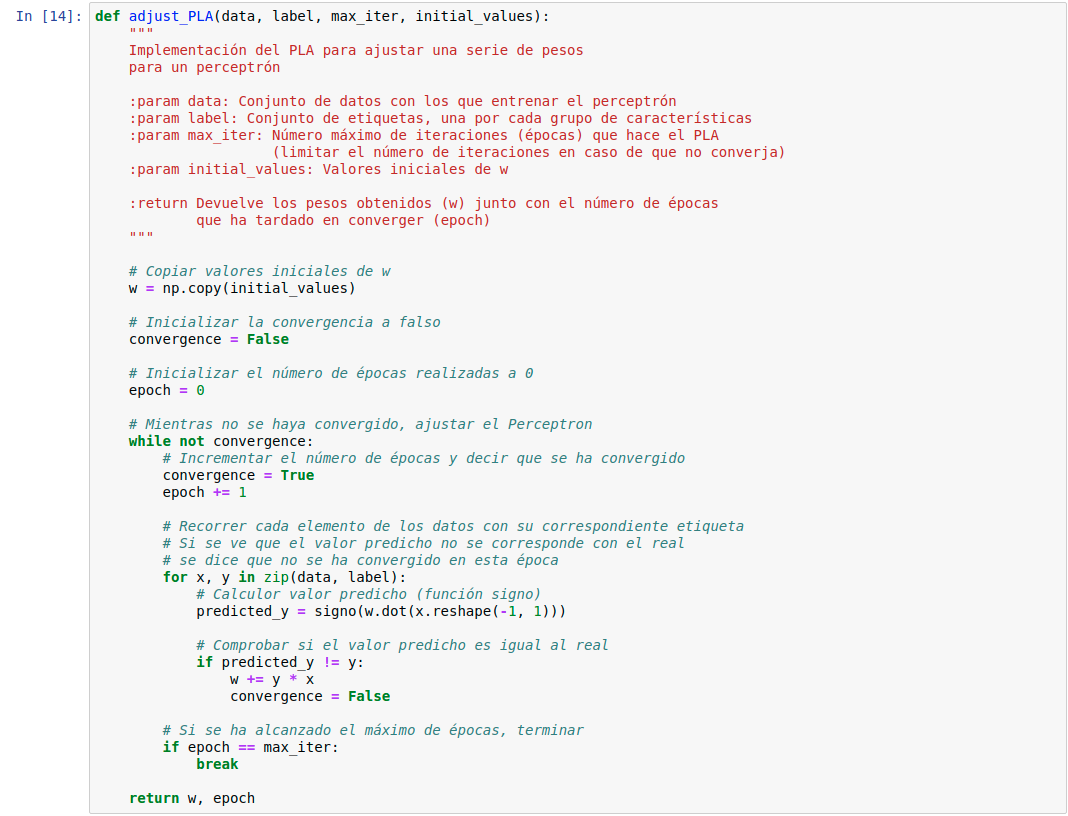
\includegraphics[scale=0.4]{img/adjust_pla.png}
\caption{Implementación de la función $ajusta\_PLA()$.}
\end{figure}

\begin{enumerate}[label=\textit{\alph*})]
	\item Ejecutar el algoritmo PLA con los datos simulados en los apartados 2\textit{a} de la
	sección.1. Inicializar el algoritmo con: a) el vector cero y, b) con vectores de números
	aleatorios en $[0, 1]$ (10 veces). Anotar el número medio de iteraciones necesarias en ambos para
	converger. Valorar el resultado relacionando el punto de inicio con el número de iteraciones.
\end{enumerate}

Los resultados de ejecutar el algoritmo con los distintos datos son los siguientes:

\begin{figure}[H]
\centering
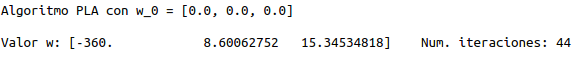
\includegraphics[scale=0.6]{img/pla_0_normal.png}
\caption{Resultado del algoritmo PLA con un $w_0 = [0, 0, 0]$.}
\end{figure}

Como se puede comprobar, la haber partido de $w_0 = [0, 0, 0]$, el algoritmo PLA tarda 44 iteraciones
(es decir, 44 épocas, o lo que es lo mismo, 44 vueltas completas a los datos) en converger.

\begin{figure}[H]
\centering
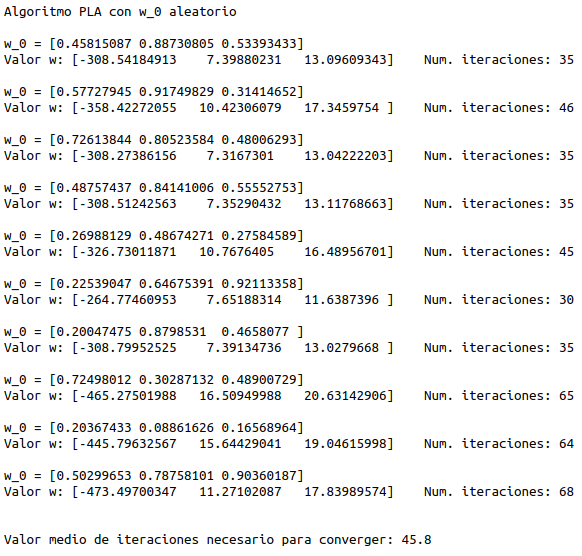
\includegraphics[scale=0.52]{img/pla_rand_normal.png}
\caption{Resultado del algoritmo PLA con un $w_0$ aleatorio.}
\end{figure}

En este caso, aunque no se especificaba, también se ha mostrado individualmente cuánto tarda el
algoritmo PLA en converger para cada punto aleatorio. En algunos casos tarda más que en otros, debido
a que estos puntos pueden estar más cerca del correspondiente plano obtenido, pero de media se tarda
$45.8$ épocas en converger. Este valor medio se queda muy cerca de las 44 épocas anteriores, con
lo cuál, a grandes rasgos, podemos decir que de media todos los valores aletorios se comportan casi
igual que un vector de pesos inicializado a 0. Se puede ver además que, dependiendo del punto inicial,
se encuentra un plano u otro que divida a los puntos, posiblemente debido a la proximidad de estos
puntos a dicho plano, aunque en algunos casos los planos obtenidos son bastante parecidos (los que
tienen mismo número de iteracones son casi iguales). Esto no es
de extrañar, ya que existen muchísimos planos que pueden separar a los datos si estos son linealmente
separables.

Con esto podemos decir que la posición inicial de $w$ influye en el número de épocas hasta que
que el algoritmo converja, pero que si los datos son linealmente separables, como es este caso,
se llega a converger siempre, aunque sea de forma un poco lenta ya que se requieren muchas iteraciones
hasta poder converger.

\begin{enumerate}[resume,label=\textit{\alph*})]
	\item Hacer lo mismo que antes usando ahora los datos del apartado 2\textbf{b} de la sección.1.
	¿Observa algún comportamiento diferente? En caso afirmativo diga cual y las razones para que ello
	ocurra.
\end{enumerate}

Vamos a ver cuáles son los resultados obtenidos en cada caso.

\begin{figure}[H]
\centering
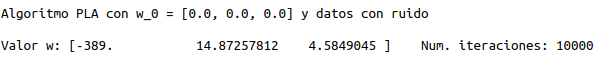
\includegraphics[scale=0.6]{img/pla_0_noise.png}
\caption{Resultado del algoritmo PLA con un $w_0 = [0, 0, 0]$ y con ruido en la muestra.}
\end{figure}

\begin{figure}[H]
\centering
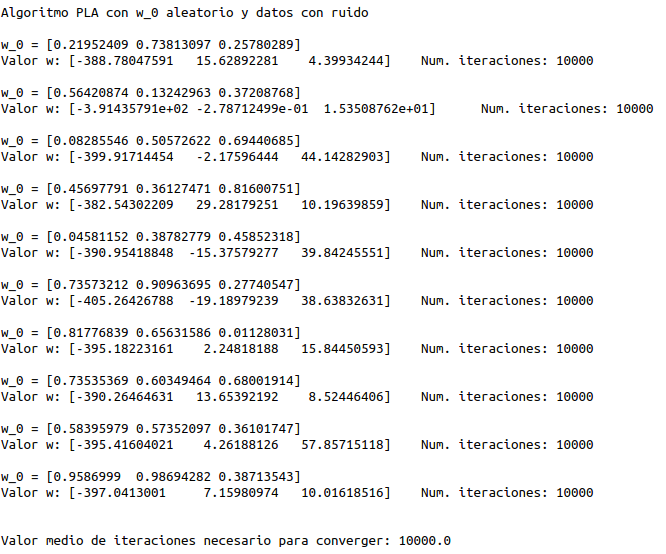
\includegraphics[scale=0.52]{img/pla_rand_noise.png}
\caption{Resultado del algoritmo PLA con un $w_0$ aleatorio y con ruido en la muestra.}
\end{figure}

Como se puede comprobar a simple vista, todos los algoritmos terminan en el mismo número de
iteraciones. No es casualidad, ya que al algoritmo se le ha especificado que $max\_iter$ sea
10000 iteraciones o épocas. Entonces, ¿por qué sucede esto?

La respuesta es muy simple, y es que los datos no son linealmente separables. En los datos con ruido
hay puntos de una clase que están mezclados con los de la otra, y no existe ninguna forma de
separar esos datos con una recta/plano (habría que intentar utilizar algo más complejo como una
circunferencia o una elipse, aunque tampoco se garantiza que se consiga algo con estos, aparte de
que el PLA solo trabaja con planos/rectas). Por tanto, el algoritmo PLA nunca va a poder converger en
estos casos, que es precisamente lo que sucede en este ejemplo.

\subsection*{Apartado 2}
\addcontentsline{toc}{subsection}{Apartado 2}

\noindent \textbf{Regresión Logística}: En este ejercicio crearemos nuestra propia función
objetivo $f$ (una probabilidad en este caso) y nuestro conjunto de datos $\mathcal{D}$ para ver cómo
funciona regresión logística. Supondremos por simplicidad que $f$ es una probabilidad con
valores $0/1$ y por tanto que la etiqueta $y$ es una función determinista de $\mathbf{x}$.

\noindent Consideremos $d = 2$ para que los datos sean visualizables, y sea
$\mathcal{X} = [0, 2] \times [0, 2]$ con probabilidad uniforme de elegir cada
$\mathbf{x} \in \mathcal{X}$ . Elegir una línea en el plano que pase por $\mathcal{X}$
como la frontera entre $f(\mathbf{x}) = 1$ (donde $y$ toma valores $+1$) y $f(\mathbf{x}) = 0$
(donde $y$ toma valores $-1$), para ello seleccionar dos puntos aleatorios del plano y calcular la
línea que pasa por ambos. Seleccionar $N = 100$ puntos aleatorios $\lbrace \mathbf{x}_n \rbrace$
de $\mathcal{X}$ y evaluar las respuestas $\lbrace y_n \rbrace$ de todos ellos respecto de la frontera
elegida.

Para generar los datos, vamos a utilizar la función $simula\_unif()$ y la función $simula\_recta()$,
las cuales han aparecido anteriormente. Aparte de esto, hemos cambiado la semilla aleatoria que se
proporcionaba al principio, ya que los datos que se generaban inicialmente, junto con la recta, no
eran muy buenos. Esta creación se puede comprobar en el siguiente código:

\begin{figure}[H]
\centering
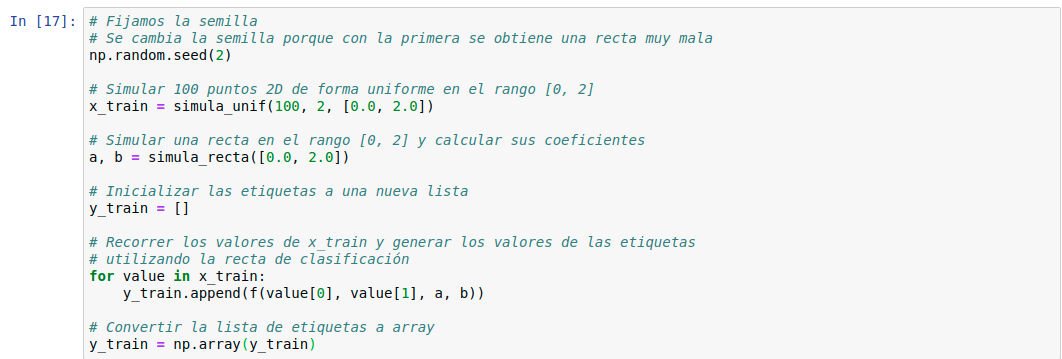
\includegraphics[scale=0.4]{img/init_data.png}
\caption{Código para generar los datos iniciales.}
\end{figure}

Una vez generados, al representar la muestra con las etiquetas correspondientes y con la recta
$f$ que divide en dos clases, obtenemos la siguiente gráfica:

\begin{figure}[H]
\centering
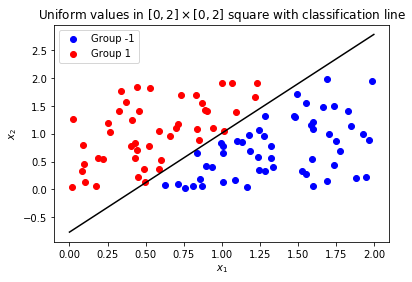
\includegraphics[scale=0.6]{img/regression_1.png}
\caption{Gráfica de los datos generados para el problema de Regresión Lineal.}
\end{figure}

\begin{enumerate}[label=\textit{\alph*})]
	\item Implementar Regresión Logística (RL) con Gradiente Descendente Estocástico (SGD)
	bajo las siguientes condiciones:
	
	\begin{itemize}
		\item Inicializar el vector de pesos con valores 0.
		\item Parar el algoritmo cuando
		$||\mathbf{w}^{(\text{t}-1)} - w^{(\text{t})} || < 0.01$, donde $w^{(\text{t})}$ denota el
		vector de pesos al final de la época $t$. Una época es un pase completo a través de los $N$
		datos.
		\item Aplicar una permutación aleatoria, $1, 2, \dots , N$, en el orden de los datos antes de
		usarlos en cada época del algoritmo.
		\item Usar una tasa de aprendizaje de $\eta = 0.01$.
	\end{itemize}
\end{enumerate}

A continuación se procede a mostrar la implementación de Regresión Lineal con Gradiente Descendente
Estocástico:

\begin{figure}[H]
\centering
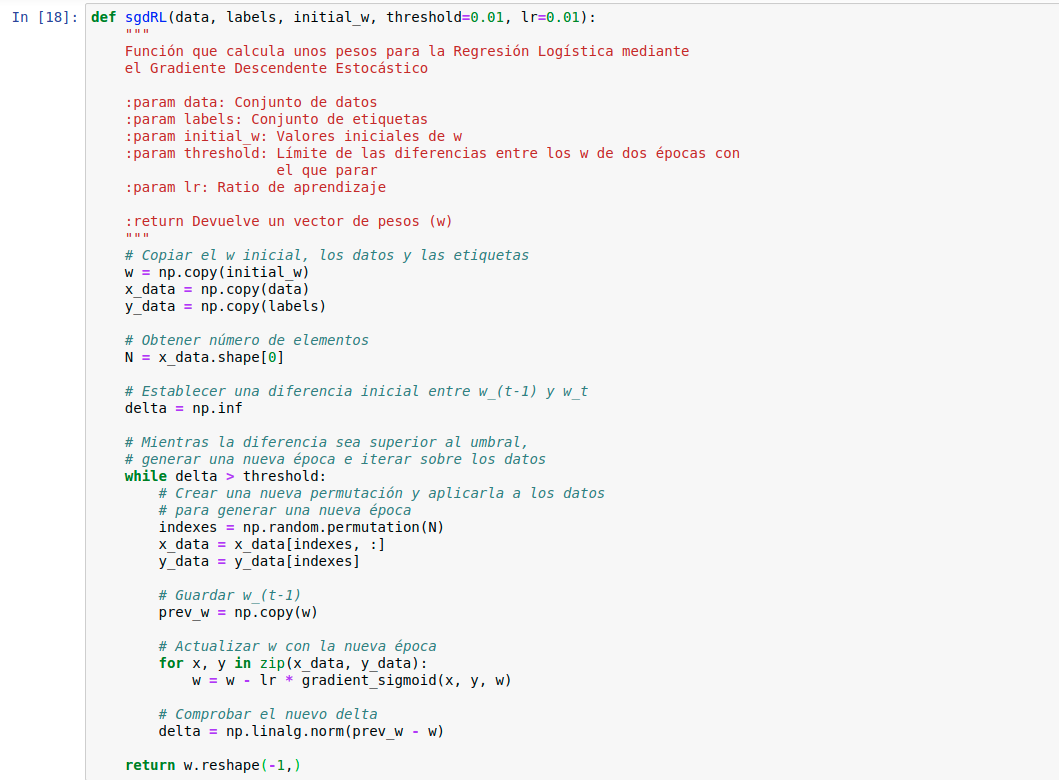
\includegraphics[scale=0.4]{img/sgdRL.png}
\caption{Implementación de Regresión Lineal mediante SGD.}
\end{figure}

Esta implementación genera, para cada época, una nueva permutación de los datos, y actualiza $w$ con
un batch de tamaño 1, recorriendo todos los datos. Se ha llamado $delta$ a la diferencia
$||\mathbf{w}^{(\text{t}-1)} - w^{(\text{t})} ||$, es decir, a la distnacia Euclídea entre los
dos vectores de pesos, y para calcularla se ha usado una función de \textit{numpy} que se encarga
de eso.

También se ha utlizado una función que calcula el gradiente del sigmoide, el cuál viene dado por la
siguiente expresión:

\begin{equation}
	\nabla E_{\text{in}} = - \frac{1}{N}
	\sum_{n = 1}^N \frac{y_n\mathbf{x}_n}{1 + e^{y_n\mathbf{w}^{\text{T}}\mathbf{x}_n}}
\end{equation}

Como el \textit{batch} es de tamaño 1, la expresión anterior queda de la siguiente forma:

\begin{equation}
	\nabla E_{\text{in}} = - \frac{y_n\mathbf{x}_n}{1 + e^{y_n\mathbf{w}^{\text{T}}\mathbf{x}_n}}
\end{equation}

Este resultado se puede ver en el siguiente código:

\begin{figure}[H]
\centering
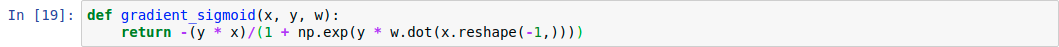
\includegraphics[scale=0.4]{img/gradient_sigmoid.png}
\caption{Implementación del gradiente de la función sigmoide.}
\end{figure}

Con los datos generados anteriormente, y pasándole un vector de pesos inicializado a 0 cada
componente, se obtiene la siguiente gráfica:

\begin{figure}[H]
\centering
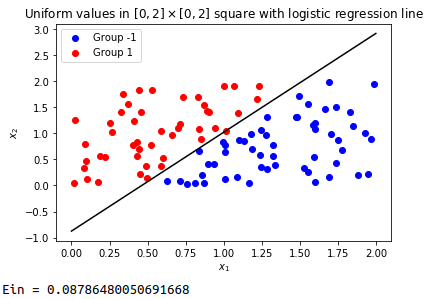
\includegraphics[scale=0.6]{img/regression_2.png}
\caption{Recta de Regresión Lineal ajustada mediante SGD junto con \ein.}
\end{figure}

Como se puede ver, se ha obtenido una recta casi idéntica a la anterior, solo que un poquito más
inclinada (esto se puede notar en uno de los puntos rojos que corta, como lo deja casi por encima de
la recta). Como se puede observar, el valor de \ein{} es bastante pequeño, con lo cuál el ajuste
realizado es muy bueno.  Para calcular este error, se ha utilizado la siguiente fórmula, la cuál
sigue el criterio ERM:

\begin{equation}
	\label{eq:ein_erm}
	E_{\text{in}} = \frac{1}{N}
	\sum_{i = 0}^N \ln \Big( 1 + e^{-y_i\mathbf{w}^\text{T}\mathbf{x}_i}  \Big)
\end{equation}

El motivo por el que el \ein{} no es exactamente 0 si no un valor muy pequeño se debe al exponente.
Cuando los datos son clasificados correctamente, el valor del exponente es negativo (por el signo
negativo delante de $y_i$), con lo cuál esa exponenciación tendrá un valor pequeño, aunque no tan
pequeño como para que el logaritmo neperiano de la suma sea 0, si no un poco mayor. Si los datos
no son clasificados correctamente, el valor de la exponenciación es positivo, y por tanto esa
suma dentro del logaritmo se hace mucho mayor, incrementando en mayor medida el error.

Una vez comentado ese aspecto, se procede a mostrar la implementación de la función para calcular
el error en una muestra:

\begin{figure}[H]
\centering
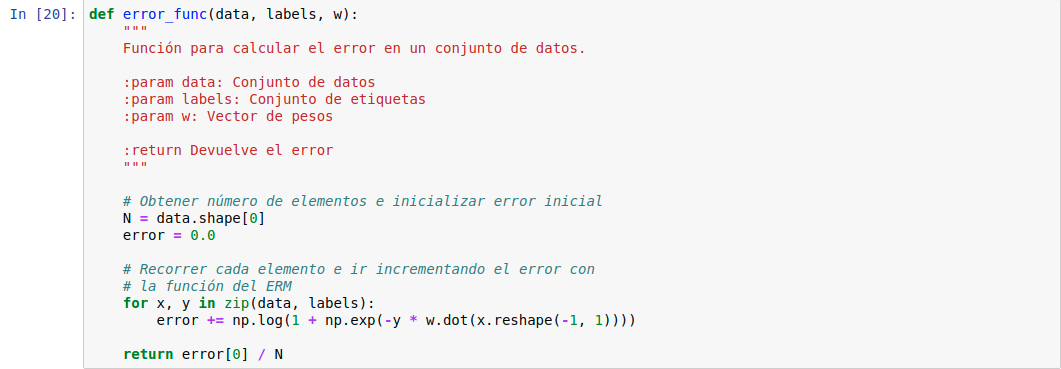
\includegraphics[scale=0.4]{img/error_func.png}
\caption{Implementación de la función de error con el criterio ERM \eqref{eq:ein_erm}.}
\end{figure}

\begin{enumerate}[resume,label=\textit{\alph*})]
	\item Usar la muestra de datos etiquetada para encontrar nuestra solución $g$ y estimar 
	\eout{} usando para ello un número suficientemente grande de nuevas muestras (>999).
\end{enumerate}

Para este experimento, se ha generado una muestra aleatoria con la función $simula\_unif()$ con
$N = 2500$, la cuál se puede ver a continuación:

\begin{figure}[H]
\centering
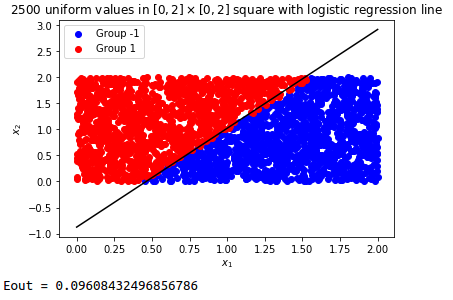
\includegraphics[scale=0.6]{img/regression_3.png}
\caption{Muestra de 2500 elementos con la recta de Regresión Logística y el valor de \eout{}.}
\end{figure}

Como se puede ver, la recta divide casi perfectamente a la nueva muestra, a excepción de algunos
puntos rojos que parece que están más pegados a los azules, quedando al otro lado de la zona de
la recta que clasifica a los puntos rojos con la etiqueta $+1$.
Sin embargo, al observar el valor de \eout{}, podemos ver que el ajuste es muy bueno, ya que este
error es solo una centésima superior al valor de \ein{}, con lo cuál ambos valores están muy próximos.
De aquí podemos sacar que la muestra que teníamos de entrenamiento representa muy bien a la población
y tenía el tamaño suficiente como para poder entrenar correctamente a nuestro modelo.

\end{document}

